\documentclass[times, utf8, seminar]{fer}
\usepackage{booktabs}
\usepackage{framed}
\usepackage[tikz]{bclogo}
\usepackage{amsmath}
\usepackage{hyperref}
\usepackage{multirow}
\usepackage{amssymb}
\usepackage[scaled]{beramono}
\usepackage{listings}
\usepackage{algorithmicx}
\newcommand{\argmax}{\arg\!\max}
\makeatletter
\lstset{
  language={Python},
  basicstyle=\footnotesize
}
\begin{document}

% TODO: Navedite broj rada.

% TODO: Navedite naslov rada.
\title{Gibbsovo uzorkovanje}

% TODO: Navedite vaše ime i prezime.
\author{Filip Boltužić}
\voditelj{Prof. dr. sc. Bojana Dalbelo Bašić}
\maketitle

\tableofcontents

\chapter{Uvod}
Gibbsovo uzorkovanje pripada Monte Carlo Markovljevim \engl{Monte Carlo Markov Chain, MCMC} metodama. Markovljevim lancima modelira se bezmemorijski matematički sustav stanja i prijelaza između stanja \citep{kass1998markov}. Markovljev lanac je niz vrijednosti generiranih u procesu s Markovljevim svojstvom. Prema Markovljevom svojstvu međuovisnost postoji samo između susjednih vrijednosti, tj. vrijednost u Markovljevom lancu generira se samo na temelju prethodne vrijednosti, zbog čega se nazivaju bezmemorijskim. 

Gibbsovo uzorkovanje zadovoljava obilježja Monte Carlo metoda i Markovljevih lanaca. Metoda generira niz uzoraka, gdje su generirani susjedi međusobno zavisni (korelirani). Početni uzorci \engl{burn out period} Gibbsovog uzorkovanja se često zanemaruju jer ne predstavljaju ciljanu distribuciju.


%%KRAJ UVODA

\section{Pretpostavke}

Distribucija iz koje je potrebno uzorkovati je "posebna", jer nije moguće uzorkovati izravno. Izračun vjerojatnosti sunčanog ili kišovitog vremena tijekom sutrašnjeg dana proces je koji je moguće procijeniti Gibbsovim uzorkovanjem. No, informacije koje su potrebne za Gibbsovo uzorkovanje su informacije o uvjetnim distribucijama vjerojatnosti sunčanog, odnosno kišovitog vremena. Potrebno je poznavati vjerojatnosti o vremenu temeljem današnjeg vremena. Odnosno, ukoliko nas zanimaju $P(sutra = ki$š$a)$ i $P(sutra = sunce)$, potrebno je poznavati vjerojatnosti:
\begin{itemize}
\item $P(sutra = ki$š$a | danas = ki$š$a)$
\item $P(sutra = ki$š$a | danas = sunce)$
\item $P(sutra = sunce | danas = ki$š$a)$
\item $P(sutra = sunce | danas = sunce)$
\end{itemize}



\chapter{Monte Carlo metode}

\section{Povijest}

Monte Carlo metode obuhvaćaju računalne modele zasnovane na stohastičkoj matematici, točnije, uporabi nasumičnih brojeva u izračunima. Moderne Monte Carlo metode osmislio je Stanislaw Ulam \citep{kass1998markov}, a ime su dobile po omiljenom odredištu zabave Ulamovog ujaka -- Monte Carlo kockarnicama. Originalno su zamišljene kako bi pomogle pri difuziji neutrona. Svrha Monte Carlo metoda bila je izraditi umjetno stvoriti nasumičan proces bez mogućnosti upravljanja njime. John von Neumann, slavni znanstvenik, uvidio je potencijal Monte Carlo metode i implementirao ih na računalu ENIAC. Intenzivnija primjena Monte Carlo metoda počela je s pojavom snažnijih računala. 

\section{Mehanizam}

Monte Carlo metode pokušavaju oponašati slučajne procese u prirodi (npr. bacanje novčića). Na taj način pokušavaju se predvidjeti svi mogući ishodi i vjerojatnosti događaja unutar okvira zadanog procesa. 

Monte Carlo metoda je probabilistički računalni algoritam koji pokušava predvidjeti sve moguće ishode i vjerojatnosti procesa na koji je primijenjen. Temelji se na slučajnim varijablama, koje je potrebno zadati u obliku funkcije gustoće \citep{gilks1996markov}. Na temelju funkcija gustoće $P(x)$ Monte Carlo metodama moguće je riješiti probleme:
\begin{itemize}
\item generiranja $R$ uzoraka $\{x^{(r)}\}_{r=1}^{R}$ iz $P(x)$,
\item izračun očekivanja funkcija s distribucije $P(x)$.
\end{itemize}


Monte Carlo metodama se simuliraju sustavi s mnogo neizvjesnosti. Pokazale su se iznimno učinkovite prilikom modeliranja složenih vjerojatnosti i strategija odlučivanja kojima nije moguće upravljati, ili ih je iznimno teško ili zahtjevno izgraditi. Izračun osiguranja, modeliranje kreditnih rizika u financijskim institucijama, rekonstrukcija eksplozija samo su neki primjeri u kojima se koriste Monte Carlo metode, zbog činjenice da je navedene procese u stvarnosti teško simulirati i pratiti. 

U Monte Carlo analizama potrebno je definirati distribucije vjerojatnosti slučajnih varijabli. Markovljevim lancima moguće je modelirati međuovisnost, što nije moguće Monte Carlo metodama. Ukoliko je potrebno dobiti uzorke iz aposteriori distribucije vjerojatnosti, Markovljevim lancima moguće je uzastopno uzorkovati dok uzorkovanje ne postane stabilan proces. Tada je moguće dobiti nezavisne uzorke iz aposteriori distribucije vjerojatnosti. 

Monte Carlo integracija pripada Monte Carlo metodama, a služi za izračun integrala. 

Monte Carlo metode imaju svojstvo crne kutije \engl{black box}. Njima je moguće dobiti odgovore na razna pitanja procjene vjerojatnosti, kao: kolika je vjerojatnost kiše sutra, kolika je vjerojatnost da će Googleova dionica izgubiti na vrijednosti, kolika je vjerojatnost da će klijent vratiti kredit \dots No, nije moguće saznati koji su razlozi na temelju kojih je dobivena određena vjerojatnost. 

\chapter{Markovljev lanac}

Markovljeve lance inicijalno je predstavio ruski znanstvenik Andrey Markov 1912. godine. Markov je pokušao modelirati slavno remek djelo Aleksandra Puškina \textit{Jevgenij Onjegin}. Cilj modela bio je predviđanje idućih slova temeljem trenutnih. Markovljeva ideja je po prvi puta predstavila koncepte zavisne varijable i uvjetne vjerojatnosti.

\begin{figure}
\centering
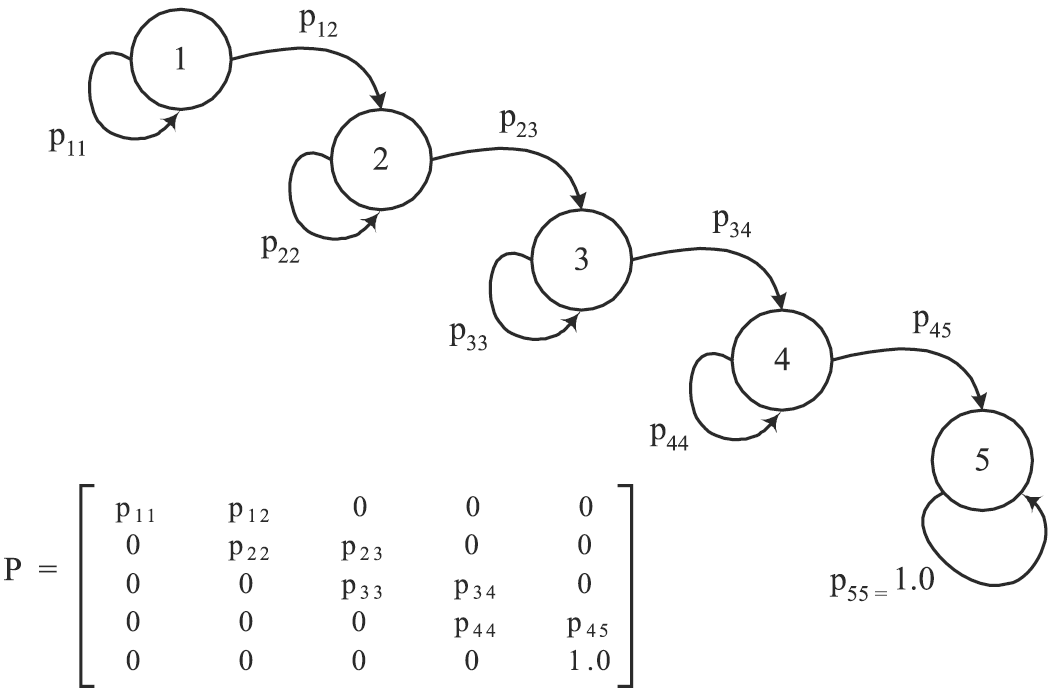
\includegraphics[scale=1]{markov_chain_example.png}
\caption{Primjer Markovljevog lanca. Preuzeto iz \citep{wirahadikusumah2003application}.}
\label{fig:markov_example}
\end{figure}

Markovljevi lanci se, također, primjenjuju nad širokim spektrom problema. Koriste se za modeliranje događaja i njihovih vjerojatnosti kada nije potrebno pamtiti prošle događaje. Markovljevi lanci sastoje se od niza stanja i vjerojatnosti prijelaza između stanja. Primjer Markovljevog lanca prikazan je slikom \ref{fig:markov_example}. Na slici je vidljivo pet stanja označenim brojevima u krugovima, jednosmjernih strelica kojima se označavaju mogućih prijelazi te matrica prijelaza $P$, matrični zapis Markovljevog lanca. Markovljev lanac ima oblik usmjerenog grafa. Stanja na burzama dionica, vremenska prognoza, prepoznavanje govora su neke od problema koji se često modeliraju Markovljevim 
lancima. 

Markovljevi lanci pretpostavljaju kako je sustav koji se modeliraju stabilan. U praksi, to često nije tako. Kompleksni sustavi, kao što su burze dionica,  sastoje se od pravilnosti i šuma. No, često moguće procijeniti jesu li vjerojatnosti dobivene danas relevantne za nekoliko godina.

\chapter{Gibbsovo uzorkovanje}
\label{cha:gibbs_dsc}
Gibbsovo uzorkovanje je dobilo ime po Josiahu Willardu Gibbsu, američkom znanstveniku 19. stoljeća koji je izumio Gibbsova nasumična polja. Stuart i Donald Geman su prvi puta opisali postupak Gibbsovog uzorkovanja \citep{geman1984stochastic}. Braća Geman bavili su se izradom modela za analizu slike. Gibbsovo uzorkovanje u njihovom radu je poseban slučaj Metropolis-Hastings algoritma \citep{metropolis1953equation}. \citep{gelfand1990sampling} su pokazali potencijalne primjene Gibbsovog uzorkovanja prilikom rješavanja velikog broja statističkih problema.

Gibbsovo uzorkovanje koristi Monte Carlo tehnike za procjenu vjerojatnosti u modelu zasnovanom na Markovljevom lancu. Prema tome, Gibbsovo uzorkovanje primjenjuje se u kompleksnim sustavima visokog stupnja entropije, gdje pretpostavljamo da iduće stanje ovisi samo o trenutnom stanju. Najčešće se koristi za izračune vrijednosti određenih integrala, posebice u višedimenzionalnim slučajevima. 

Metropolis Hastings algoritam sličan je algoritmu Gibbsovog uzorkovanja. Metropolis Hastings algoritam ne donosi odluke temeljem svih uvjetnih distribucija vjerojatnosti, već donosi odluku o prihvaćanju ili odbijanju učinjenog koraka (odbijanje vodi u prethodni korak). 

Ako je moguće dobiti nezavisne uzorke izravno iz distribucije, dovoljno je koristiti Monte Carlo mehanizme. Ukoliko su poznate samo uvjetne vjerojatnosti, a potrebno je uzorkovati iz zajedničke distribucije vjerojatnosti nužno je koristiti Metropolis Hastings algoritam ili Gibbsovo uzorkovanje. Gibbsovo uzkorkovanje daje uzorak za svaki korak, ali zahtjeva potpunu informaciju o uvjetnim distribucijama vjerojatnosti, što Metropolis Hastings algoritam ne zahtjeva, već odbacuje dobivene uzorke ukoliko su dobiveni na temelju izrazito niske vjerojatnosti. 

Gibbsovo uzorkovanje neće uvijek konvergirati. 

\chapter{Metoda Gibbsovog uzorkovanja}
Zajednička distribucija \engl{joint distribution} definirana je jednadžbom:

\begin{equation} \label{eq:joint distribution}
f(x, y_1, y_2, \dots , y_p).
\end{equation}
Potrebno je izračunati svojstva marginalne distribucije \engl{marginal distribution}
\begin{equation} \label{eq:marginal distribution}
f(x) = \int \dots \int f(x,y_1, y_2, \dots , y_p) dy_1 dy_2 \dots dy_p
\end{equation}
kao što su srednja vrijednost \engl{mean} ili standardna devijacija \engl{standard deviation}. Analitičkim izračunom integrala \ref{eq:marginal distribution} dobije se $f(x)$, nakon čega je moguće izračunati željena svojstva. Analitički (ili numerički) izračun integrala može biti izuzetno složen. Gibbsovo uzorkovanje je alternativan način računjanja marginalne distribucije $f(x)$.

Gibbsovim uzorkovanjem generiraju se uzorci $X_1, ..., X_m ~ f(x)$ bez poznate funkcije $f(x)$. Generiranjem dovoljno velikog uzorka, moguće je izračunati svojstva, kao što su srednja vrijednost ili standardna devijacija, funkcije $f(x)$ s određenom preciznošću. 

\section{Dvodimenzionalni slučaj}

Prvi primjer Gibbsovog uzorkovanja bit će objašnjen za dvodimenzionalni slučaj. Gibbsovim uzorkovanjem se za par slučajnih varijabli $(X,Y)$ želi dobiti $f(x)$. Poznate su uvjetne distribucije $f(x|y)$ i $f(y|x)$. Generira se Gibbsova sekvenca:
\begin{equation} \label{eq:gibbs sequence}
Y_{0}^{'}, X_{0}^{'}, Y_{1}^{'}, X_{1}^{'}, \dots , Y_{k}^{'}, X_{k}^{'}. 
\end{equation}
Postavlja je inicijalna vrijednost $Y_{0}^{'} = y_{0}^{'}$, dok se sve ostale vrijednosti generiraju prema

\begin{align} \label{eq:gibbs step condition}
X_{j}^{'} \sim f(x | Y_{j}^{'}=y_{j}^{'}) \nonumber \\
Y_{j+1}^{'} \sim f(y | X_{j}^{'} = x_{j}^{'}).
\end{align}

Generiranje niza \eqref{eq:gibbs sequence} prema formuli \eqref{eq:gibbs step condition} naziva se \textbf{Gibbsovo uzorkovanje}. \citep{gelfand1990sampling} su predložili generiranje $m$ nezavisnih Gibbsovih sekvenci duljine $k$. Posljednje vrijednosti $X_{k}^{'}$ svake od $m$ sekvenci se potom koriste za aproksimaciju $f(x)$. Ako je $k$ dovoljno velik, uzorak $X^{'}$ je nezavisna i jednako distribuirana varijabla \engl{independent and identically distributed} kao i inicijalna nasumična varijabla $X$. Primjere dvodimenzionalnog slučaja Gibbsovog uzorkovanja pokazali su \citep{casella1992explaining}.

\subsection{Primjer 1}

Primjer zajedničke distribucije nasumičnih varijabli $X$ i $Y$:
\begin{align} \label{eq:example1}
f(x,y) \propto {n \choose x} y^{x + \alpha - 1}(1-y)^{n - x + \beta - 1}, \nonumber \\
x = 0,1, \dots ,n \nonumber \\
0 \le y \le 1.
\end{align}

Potrebno je izračunati svojstva marginalne distribucije $f(x)$ slučajne varijable $X$. Uvjetne distribucije su poznate:

\begin{subequations} 
\begin{align} 
f(x|y) = {n \choose k}\, y^k (1-y)^{n-k} \label{eq:example1a} \\
f(y|x) = \frac{\Gamma(\alpha+n + \beta)}{\Gamma(x + \alpha)\Gamma(n - x + \beta)}\, y^{x + \alpha-1}(1-y)^{n - x + \beta-1} \label{eq:example1b}
\end{align}
\end{subequations}

Generiranjem Gibbsove sekvence formulom \eqref{eq:gibbs step condition} pomoću uvjetnih distribucija \eqref{eq:example1a} i \eqref{eq:example1b} dobivaju se $X_1, X_2, \dots ,X_m$ iz $f(x)$. Dobiveni $f(x)$ je aproksimacija pravog $f(x)$ kojeg je moguće analitički ili numerički izračunati iz zajedničke distribucije \eqref{eq:example1}. U ovome primjeru analitičkim izračunom dobiva se da je
\begin{align}
f(x) = {n \choose x} \frac{\Gamma(\alpha+\beta)}{\Gamma(\alpha)\Gamma(\beta)}\frac{\Gamma(x+\alpha)\Gamma(n-x+\beta)}{\Gamma(\alpha + \beta +n)} \nonumber \\
x = 0,1, \dots ,n.
\end{align}

Ovdje je moguće usporediti koliko je precizno Gibbsovo uzorkovanje.

\subsection{Primjer 2}

Uvjetne distribucije slučajnih varijabli $X$ i $Y$ su eksponencijalne distribucije
\begin{align}
f(x|y) \propto ye^{-yx}, 0 < x < B < \infty \nonumber \\
f(y|x) \propto xe^{-xy}, 0 < y < B < \infty,
\end{align}
gdje je $B$ poznata konstanta veća od nule. Ograničenje uvjetnih distribucija na interval $(0,B)$ je dovoljan uvjet za postojanje marginalne distribucije $f(x)$. 

Prosjek konačnih vrijednosti $Y_{k}^{'}$ i $X_{k}^{'}$ Gibbsovih sekvenci može poslužiti za izračun prave marginalne distribucije. Ako se generira $m$ sekvenci Gibbsovim uzorkovanjem onda se vrijednost f(x) može aproksimirati 
\begin{equation} \label{eq:density}
\hat{f}(x) = \frac{1}{m}	\sum_{i=1}^{m} f(x|y_i).
\end{equation}

Jednadžba \eqref{eq:density} je procjena gustoće. Prilikom izračuna $f(x)$ koristi se informacija o prethodnom stanju $y_1$, \dots ,$y_m$ iz $m$ Gibbsovih sekvenci. Procjena sadrži više informacija od procjene s vrijednostima $x_1$, \dots $x_m$. Reo-Blackwell teorem sadrži dokaz \citep{casella1996rao}.



\chapter{Dokaz konvergencije}
Potreban je dokaz da Gibbsova sekvenca \eqref{eq:gibbs sequence} proizvodi konvergentne nizove za nasumična varijabla distribucije $f(x)$. 

$X$ i $Y$ su nasumične varijable, sa zajedničkom raspodjelom

\begin{equation}
\begin{bmatrix}
f_{x,y}(0,0) & f_{x,y}(1,0) \\
f_{x,y}(0,1) & f_{x,y}(1,1) 
\end{bmatrix} 
= 
\begin{bmatrix}
p_1 & p_2 \\
p_3 & p_4
\end{bmatrix}
\end{equation}

Marginalna distribucija $x$ je
\begin{equation}
f_x = \begin{bmatrix}
f_x(0) & f_x(1)
\end{bmatrix}
= \begin{bmatrix}
p_1 + p_3 & p_2 + p_4.
\end{bmatrix}
\end{equation}

Prema tome, uvjetne distribucije $X|Y=y$ i $Y|X=x$ iznose:
\begin{align} \label{eq:matrix conditional distributions}
A_{y|x} = \begin{bmatrix}
\frac{p_1}{p_1+p_3} & \frac{p_3}{p_1+p_3} \\
\frac{p_2}{p_2+p_4} & \frac{p_4}{p_2+p_4}
\end{bmatrix},
A_{x|y} = \begin{bmatrix}
\frac{p_1}{p_1+p_2} & \frac{p_2}{p_1+p_2} \\
\frac{p_3}{p_3+p_4} & \frac{p_4}{p_3+p_4}
\end{bmatrix}
\end{align}

Dobivene matrice sliče matricama prijelaza karakterističnim za Markovljeve lance \citep{gilks1996markov}. Generiranje Gibbsove sekvence \eqref{eq:gibbs sequence} zahtjeva uvjetne distribucije, što je prikazano \eqref{eq:matrix conditional distributions}. U ovom slučaju Gibbsova sekvenca bit će niz nula i jedinica. Prema \eqref{eq:gibbs step condition} potrebno je povezati uvjetne distribucije za dobivanje koraka Gibbsove sekvence, iz čega nastaje

\begin{equation}
P(X^{'}_{1}=x_1 | X^{'}_{0}=x_0) = \sum_{y} P(X^{'}_{1} | Y^{'}_{1}=y_1) \cdot P(Y^{'}_{1}=y_1|X^{'}_{0}=x_0)
\end{equation}, 
u matričnom obliku
\begin{equation}
A_{x|x} = A_{y|x}A{x|y}.
\end{equation}

Vrijedi:
\begin{equation} \label{eq:induction}
f_k = f_0 A_{x|x}^{k} = (f_0 A_{x|x}^{k-1})A_{x|x} = f_{k-1} A_{x|x}
\end{equation}

Korak $k$ Gibbsove sekvence se dobije kao $(A_{x|x}^{k}$. Ako su vrijednosti u $A_{x|x}$ pozitivne, onda \eqref{eq:induction} za bilokoju inicijalnu vjerojatnost $f_0$ i kada $k \to \infty$, $f_k$ konvergiira distribuciji $f$ koja je stacionarna točna niza \eqref{eq:induction} i zadovoljava jednakost
\begin{equation}
fA_{x|x}=f.
\end{equation}

Ako se generiranje Gibbsove sekvence zaustavi kod dovoljno velikog broja koraka $k$, pretpostavlja se kako je distribucija $X^{'}_{k}$ približno $f_x$. 

Sve navedeno ne vrijedi samo u slučaju $2x2$, već i u općem slučaju slučajnih varijabli $X$ i $Y$ s $n$ i $m$ mogućih vrijednosti.

\section{Matematika za slučaj dvije varijable}

Dvije slučajne varijable $X$ i $Y$. Poznate su uvjetne vjerojatnosti $f_{X|Y}(x|y)$ i $f_{Y|X}(y|x)$. Moguće je izračunati marginalnu distribuciju varijable $X$: $f_X(x)$, kao i zajedničku distribuciju $X$ i $Y$ preko:
\begin{equation}
f_X(x) = \int f_{XY}(x,y) dy,
\end{equation}
gdje je $f_{XY}(x,y)$ zajednička distribucija. 
\begin{equation}
f_{XY}(x,y) = f_{X|Y}(x|y) f_Y(y)
\end{equation}

\begin{align*}
f_X(x) &= \int f_{X|Y}(x|y)f_Y(y)dy
\end{align*}
\begin{align*}
f_X(x) &= \int f_{X|Y}(x|y) \int f_{Y|X}(y|t)f_X(t)dt dy \\
&= \int \bigg[ \int f_{X|Y}(x|y)f_{Y|X}(y|t)dy \bigg] f_X(t)dt \\
&= \int h(x,t) f_X(t) dt,
\end{align*}
gdje je 
\begin{equation}
h(x,t) = \bigg[\int f_{X|Y}(x|y)f_{Y|X}(y|t)dy\bigg].
\end{equation}

\section{Slučaj s više od dvije varijable}
U slučaju više od dvije varijable generiranje Gibbsove sekvence radi se uzorkovanje supstitucijom \engl{substitution sampling}. 

U slučaju dvije varijable uzorkovanje supstitucijom je uvijek isto. 

Za tri slučajne varijable $X$, $Y$ i $Z$ potrebno je izračunati marginalnu distribuciju $f_X(x)$. Ako se $Y$ i $Z$ promatraju kao jedna varijabla moguće je jednadžbom 
\begin{equation}
f_X(x) = \int \bigg[ \int \int f_{X|YZ}(x|y,z)f_{YZ|X}(y,z|t)dydz \bigg] f_X(t)dt
\end{equation}
izračunati marginalnu distribuciju. Gibbsova sekvenca bi za j-ti korak bila:
\begin{align*}
X_{j}^{'} \sim f(x|Y_{j}^{'} &=y_{j}^{'}, Z_{j}^{'}=z_{j}^{'}) \nonumber \\
Y_{j+1}^{'} \sim f(y|X_{j}^{'} &=x_{j}^{'}, Z_{j}^{'}=z_{j}^{'}) \nonumber \\
Z_{j+1}^{'} \sim f(z|X_{j}^{'} &=z_{j}^{'}, Y_{j+1}^{'}=y_{j+1}^{'})
\end{align*}


\chapter{Praktični dio}
Praktični dio napravljen je temeljem rada \citep{resnik2010gibbs}. Resnik i Hardisty objašnjavaju ostvarenje Naivnog Bayesa \engl{Naive Bayes} pomoću Gibbsovog uzorkovanja na primjeru klasifikacije polariteta dokumenata prema riječima u dokumentima. 

U praktičnom dijelu napravit će se sustav koji izvodi algoritam Naivnog Bayesa, a potrebne vjerojatnosti računa Gibbsovim uzorkovanjem. 

\section{Skup podataka}
\label{sec:skup}
Besplatno dostupna biblioteka \textit{Natural Language Toolkit, NLTK} \footnote{Dostupno na \url{http://www.nltk.org/} .} za programski jezik \textit{Python} sadrži pripremljene korpuse teksta. 
Za potrebe Gibbsovog uzorkovanja korišten je skup podataka \textit{movie\_reviews} koji sadrži osvrte na filmove. Format zapisa u korpusu je $<T, S>$, gdje je $T$ tekst osvrta, a $S \in \{'pos', 'neg'\}$ označeni polaritet osvrta. U nastavku će se za \textit{'pos'} kritike koristiti broj $1$, a za \textit{'neg'} kritike broj $0$. Pozitivne kritike označene su oznakom \textit{'pos'}, a negative \textit{'neg'}. Primjer negativne kritike prikazan je unutar slike \ref{fig:critic_example}.

Programski jezik korišten za \textit{Python}, verzija 2.7.3, u 64-bitnom okruženju. Dodatne \textit{Python} biblioteke korištene prilikom izrade programa su \textit{numpy}\footnote{Dostupno na \url{http://www.numpy.org/}.} i već spomenuti \textit{nltk}.

\begin{figure}
\begin{bclogo}
{Universal soldier} \footnotesize{ ex - universal soldier luc has to battle a group of newer - model engineered fighters gone bad . the review jean - claude van damme has a one - liner early on in universal soldier : the return , his latest attempt to remain relevant , that sums up this entire movie ; he says " been there , done that . " no film critic could possibly sum up van damme ' s recent film choices any better . while other ageing action stars have wisely moved into other film genres ( schwarzenegger makes as many family comedies as he does action films ) , van damme stubbornly persists in sticking with what used to work for him : martial arts and guns . this unwillingness or perhaps inability to move into new genres has caused van damme to enter the straight to video world , with legionnaire never seeing the inside of a multiplex . he joins fellow martial artist / action star steven seagal as they watch their film careers rapidly fizzle away . universal soldier : the return is truly poor . the plot is a complete copy of several action films from this decade , specifically terminator 2 : judgement day and the similarly named soldier . soldier ' s kurt russell was an older model super - soldier sent off to retirement when circumstances forced him to battle his successors , for the good of a planet ; schwarzenegger ' s terminator in t2 tried to save john connor from a newer model killing machine , the t - 1000 ; and jean - claude , a former universal soldier , has to save the planet from the rampage of a group of , you guessed it , newer model soldiers .}
\end{bclogo}
\caption{Primjer negativnog osvrta iz movie\_reviews baze podataka}
\label{fig:critic_example}
\end{figure}

\section{Matematički model}

U ovom slučaju, dokument je skup riječi koje sadrži, tzv. \engl{bag of words} princip. Za dokument $W_j$ potrebno je dodijeliti adekvatan polaritet $L_j = 0$ ili $L_j = 1$. Skup dokumenata $\mathbb{C}_{k}$ pripada skupini klase $L_j = k$, a dobije se tako da se prebroje svi dokumenti $W_j$ s $L_j=k$, prema tome $\mathbb{C}_{k} = \{W_j | L_j = k\}$. Potrebno je pronaći polaritet $L_j$ koji, za poznati dokument $W_j$, pronalazi maksimalnu vjerojatnost $P(L_j|W_J)$. Prema Bayesovom pravilu vrijedi:
\begin{equation}
L_j = \argmax_L P(L|W_j) = \argmax_L \frac{P(W_j|L)P(L)}{P(W_j)}.
\end{equation}
Moguće je izostaviti nazivnik $P(W_j)$ jer nije ovisan o $L_j$. Na ovaj način nastoji se modelirati način na koji su dokumenti nastali, što se naziva generativnim modelom \engl{Generative model}. Odabir polariteta $L_j$ modelira se Bernoulijevom raspodjelom s parametrom $\pi$:
\begin{equation}
L_j \sim Bernoulli(\pi),
\end{equation} Potrebno za svaku poziciju riječi u dokumentu $R_i$ odabrati riječ $w_j$ temeljem distribucije vjerojatnosti riječi. Odabir distribucije vjerojatnosti iz koje se uzorkuje ovisan je dodijeljenom polaritetu dokumenta $L_j$. Moguće distribucije označavat će se $\theta_0$ i $\theta_1$. Dokument $W_j$ gradit će se temeljem multinomijalne distribucije:
\begin{equation}
W_j = Multinomijalna(R_j, \theta_{L_{j}}).
\end{equation}

Pretpostavlja se da je uzorkovanje međusobno neovisno. Distribucijama $L_j$ i $W_j$ nastoji se aproksimirati način na koji su dobiveni stvarni podaci. 

\subsection{Apriori parametri}

Gore spomenute parametre distribucija $\pi$ i $\theta$ nužno je imati prije generiranja raspodjela za $W_j$ i $L_j$. Dobivanje početnih vrijednosti za $\pi$ i $\theta$ će se dobiti iz jednolike raspodjele. Konkretno, $\pi$ će se generirati Beta distribucijom s parametrima $\gamma_{\pi 1} = 1$ i $\gamma_{\pi 2} = 1$:
\begin{equation}
\pi \sim Beta(\gamma_{\pi}).
\end{equation}
Parametri apriori vrijednosti nazivaju se hiperparametrima. Kako oba parametra Beta distribucije ovdje iznose 1, svi događaji su jednako vjerojatna, što znači da je apriori znanje o sustavu nedostupno. U slučaju $\theta$ parametra, on je modeliran Dirichlechtovom distribucijom, generaliziranom Beta distribucijom važećoj u više od dvije dimenzije:
\begin{equation}
\theta \sim Dirichlet(\gamma_{\theta})
\end{equation}

\subsection{Zajednička distribucija}

Prostor stanja u ovom problemu sastoji se skalarne varijable parametra $\pi$, dva parametarska vektora $\theta_1$ i $\theta_2$, oznaka klase $L_N$ (za svaki od $N$ dokumenata) i vektora $W_J$ ($J$ je broj riječi). Gibbsovo uzorkovanje kreće se kroz $k$-dimenzionalni prostor definiran ovim varijablama. Uvjetne distribucije definiraju matricu prijelaza između stanja, a zajednička distribucija je ciljna distribucija koju želimo aproksimirati. U našem slučaju zajednička distribucija iznosi:
\begin{equation}
P(\pi|\gamma_{\pi 1}\gamma_{\pi 2})P(L|\pi)P(\theta_0 | \gamma_0)P(\theta_1 | \gamma_1)P(\mathbb{C}_0|\theta_0 ,L)P(\mathbb{C}_1 | \theta_1 , L).
\end{equation}
Postupak matematičke preobrazbe dobivene jednadžbe opisan je u \citep{resnik2010gibbs}. Konačan rezultat je:
\begin{equation}
P(\mathbb{C}, L, \pi , \theta_0 , \theta_1 ; \mu) \propto \pi^{C_1+\gamma_{\pi 1}-1}(1-\pi)^{C_0 + \gamma_{\pi 0} - 1} \prod_{i=1}^{V} \theta_{0,i}^{N_{\mathbb{C_0}}(i)+\gamma_{\theta i} - 1}\theta_{1,i}^{\mathbb{C_1}}(i)+\gamma_{\theta i} - 1.
\end{equation}
Dodatno, moguće je integrirati po varijabli $\pi$ i tako reducirati zajedničku distribuciju čime se dobije konačno rješenje:
\begin{equation}
P(L, \mathbb{C}, \theta_0 , \theta_1 ; \mu) \propto \frac{\Gamma(\gamma_{\pi 1}+\gamma_{\pi 0}}{\Gamma(\gamma_{\pi 1})\Gamma(\gamma_{\pi 0})} \frac{\Gamma(C_1+\gamma_{\pi 1}\Gamma(\mathbb{C_0}+\gamma_{\pi 0})}{\Gamma(N+\gamma_{\pi 1} + \gamma_{\pi 0})} \prod_{i=1}^{V} \theta_{0,i}^{N_{\mathbb{C_0}}(i)+\gamma_{\theta i} - 1}\theta_{1,i}^{\mathbb{C_1}}(i)+\gamma_{\theta i} - 1.
\end{equation}

\subsection{Gibbsovo uzrokovanje}

Gibbsovim uzorkovanjem se u općem slučaju dodjeljuje vrijednost varijabli $Z_i$ uzorkovanjem iz uvjetne distribucije:
\begin{equation}
P(Z_i | z_i^{(t+1)}, \dots, z_{i-1}^{t+1}, \dots , z_r^{t}).
\end{equation}
Uzorkovanje vrijednosti u trenutku $(t+1)$ moguć je nakon dobivanja uzorka svih varijabli u trenutku $t$. U našem slučaju, u trenutku $t$ poznat je broj riječi u svakom dokumentu, broj dokumenata označen s negativnim odnosno pozitivnim sentimentom, broj riječi po dokumentima označenim negativnim odnosno pozitivnim sentimentom, oznake sentimenta po dokumentu i trenutne vrijednosti hiperparametara $\theta_1$ i $\theta_2$. Izračun sentimenta $L$ se dobije uzorkovanjem prema vjerojatnostima dobivenih fiksiranjem uvjetnih vjerojatnosti za $L=0$ (negativni sentiment) i $L=1$ (pozitivni sentiment). Prema tome, $L_{i}^{(t+1)}$ se računa iz uvjetne distribucije:
\begin{equation}
P(L_i|L_{1}^{t+1}, \dots , L_{i-1}^{t+1}, \dots , L_{i+1}^t{t}, L_{N}^{t},\mathbb{C}, \theta_{0}^{t}, \theta_{1}^{t}; \mu).
\end{equation}
Na sukladan način se dobiju i vrijednosti $\theta_0$ i $\theta_1$:
\begin{equation}
P(\theta_{0}^{(t+1)}|L_{1}^{(t+1)},\dots , L_{N}^{(t+1)}, \mathbb{C}, \theta_{1}^{(t)};\mu)
\end{equation} 

\begin{equation}
P(\theta_{1}^{(t+1)}|L_{1}^{(t+1)},\dots , L_{N}^{(t+1)}, \mathbb{C}, \theta_{0}^{(t+1)};\mu)
\end{equation}

\section{Programska implementacija}

\subsection{Priprema podataka}

Prilikom programske implementacije korištene su brojne biblioteke spomenute u \ref{sec:skup}. Uvoz biblioteka napravljen je kao na slici \ref{alg:import}. U skupu podataka \textit{movie\_reviews} ima 2000 osvrta i približno 32000 različitih riječi. Zbog pojednostavljena uzorkovanja i smanjivanja prostora stanja napravljen je Naivni Bayesov klasifikator te su njime izvučene najveće vjerojatnosti određene oznake za $P(L|w)$, gdje je $L$ oznaka sentimenta, a $w$ riječ. Korišteno je 500 od 32000 mogućih riječi. Deset riječi s tog popisa prikazano je slikom \ref{alg:most_info}. Primjerice, korištenje riječi seagal (glumac) u kritici znači da će vjerojatnost da je kritika biti negativna je 13.2 veća od vjerojatnosti pozitivne vjerojatnosti. Izračun tih riječi prikazan je programskim kodom na slici \ref{alg:naive_bayes}. U konačnici gradi se matrica frekvencije riječi i dokumenata (kod na slici \ref{alg:word_doc_freq}). Element $x$ na indeksu $i,j$ govori da se riječ $j$ pojavljuje u dokumentu $i$ $x$ puta. Matrica je prikazana primjerom \ref{alg:mat_word_freq}.

\begin{figure}
\lstinputlisting[language=Python, firstline=1, lastline=5]{classifier_naive_bayes.py}
\caption{Uvoz bibilioteka}
\label{alg:import}
\end{figure}

\begin{figure}
\lstinputlisting[language=Python]{most_informative.py}
\caption{Riječi s najvišim $P(L|w)$}
\label{alg:most_info}
\end{figure}

\begin{figure}
\lstinputlisting[language=Python, firstline=7, lastline=29]{classifier_naive_bayes.py}
\caption{Algoritam naivnog Bayesa koji računa $P(L|w)$}
\label{alg:naive_bayes}
\end{figure}

\begin{figure}
\lstinputlisting[language=Python, firstline=40, lastline=64]{classifier_naive_bayes.py}
\caption{Izračun matrice frekvencija riječi i dokumenata}
\label{alg:word_doc_freq}
\end{figure}

\begin{figure}
\centering
\lstinputlisting{corpus.txt}
\caption{Primjer matrice frekvencije riječi i dokumenata}
\label{alg:mat_word_freq}
\end{figure}

\subsection{Inicijalizacija}

Matrica frekvencija riječi po dokumentima i pripadajuće oznake sentimenta predstavljaju ulazni skup podataka programu Gibbsovog uzorkovanja. Idući nužni korak je dobivanje inicijalnih vrijednosti hiperparametara $\pi$ i vektora $\theta$. Zahvaljujući \textit{Pythonovim} paketima uzorkovanje iz Dirichletove distribucije moguće je provesti iznimno jednostavno. Temeljem hiperparametara uzorkuju se parametri nužni za Gibbsovo uzorkovanje. Inicijalizacija je prikazana slikom \ref{alg:hyp_params}. Gibbsovo uzorkovanje dodatno je parametrizirano ukupnim brojem iteracija, brojem iteracija odbacivanja, udaljenosti između uzoraka, objašnjenih u poglavlju \ref{cha:gibbs_dsc}.

\begin{figure}
\lstinputlisting[language=Python, firstline=215, lastline=221]{gibbs_sampler.py}
\caption{Inicijalizacija hiperparametara}
\label{alg:hyp_params}
\end{figure}



\chapter{Zaključak}
Zaključak.

\bibliography{literatura}
\bibliographystyle{fer}

\end{document}
